\documentclass{beamer}
\usetheme{Madrid}
\usepackage{booktabs}
\usepackage{graphicx}
\usepackage{listings}
\usepackage{multirow}
\usepackage{tikz}
\usepackage{pgfplots}
\pgfplotsset{compat=1.18}
\usetikzlibrary{shapes,arrows.meta,positioning}

\lstset{
  language=Python,
  basicstyle=\ttfamily\small,
  keywordstyle=\color{blue},
  stringstyle=\color{red},
  commentstyle=\color{green},
  breaklines=true
}

\title{BUS 104: Solving the Diet Problem with Google Sheets and Open Solver}
\subtitle{BUS 104: Decision Analysis and Management Science}
\author{Danko Turcic}
\titlegraphic{\includegraphics[width=5cm]{UCR-Logo.jpg}}


\begin{document}

\maketitle

\begin{frame}{Welcome to BUS 104 Adventure!}
\frametitle{Welcome to BUS 104 Adventure!}
\begin{itemize}
  \item Instructor: Danko Turcic, Operations Management Guru
  \item Time: MW 11:00 AM - 12:20 PM
  \item GitHub Repo: \url{https://github.com/dxt48/BUS-104}
  \item Case Pack: \url{https://hbsp.harvard.edu/import/1456741}
  \item Goal: Master optimization like a pro!
  \item Today: Tackle the McDonald's Diet Problem with Google Sheets + Open Solver.
  \item Engage: Grab your laptop – let’s optimize your lunch!
\end{itemize}
\end{frame}

\begin{frame}{Why Optimize Your Diet?}
\frametitle{Why Optimize Your Diet?}
\begin{itemize}
  \item Imagine eating McDonald's daily but staying healthy!
  \item Goal: Meet nutrition needs (vitamins, protein) under 2000 calories.
  \item Real-world skill: Businesses use this for cost-effective menus.
  \item Fun Fact: You’re learning tools UCR researchers use!
  \item Challenge: Can you beat the calorie limit with tasty choices?
\end{itemize}
\end{frame}


\begin{frame}[shrink]{McDonald's Diet Problem}
You want your daily diet plan to have at least 100 percent of the U.S. FDA of vitamin C, calcium; at least 50 grams of protein; and at most 2000 calories. You are wondering if this can be accomplished by eating McDonald's daily nutrition standard.
\vspace{-5pt}
\begin{table}
\footnotesize
\begin{tabular}{p{40pt}rrrrr} % Updated column count from rrrrrrrr to rrrrr
\toprule
\multirow{2}{*}{Menu Item} & \multirow{2}{*}{Price (\$)} & \multicolumn{4}{c}{McDonald's Food Facts}\\ % Updated span from 7 to 4
\cmidrule{3-6}
 &  & Cal & Protein & Vit.~C & Calcium \\
\midrule
Hamburger & 0.69 & 260 & 13 & 2 & 15 \\\hline
Big Mac & 1.99 & 560 & 25 & 2 & 25 \\\hline
Chicken Nuggets & 1.99 & 250 & 15 & 2 & 2 \\\hline
Garden Salad & 2.05 & 35 & 2 & 40 & 4 \\\hline 
Apple Pie & 0.79 & 260 & 3 & 40 & 2 \\
\bottomrule
\end{tabular}
\end{table}
\footnotesize{* Prices recorded Jan. 12, 2000 in St. Louis, Missouri}
\end{frame}

\begin{frame}{Step 1: Set Up Google Sheets}
\frametitle{Step 1: Set Up Google Sheets}
\begin{itemize}
  \item Open Google Sheets (free at sheets.google.com).
  \item Create a new spreadsheet: Name it ``DietProblem2025''.
  \item Add headers: Menu Item, Price, Calories, Protein, Vit C, Calcium.
  \item Enter data from the table – let’s build our optimization playground!
  \item Engage: Type fast – race your neighbor to finish!
\end{itemize}
\end{frame}

\begin{frame}{Step 2: Install Open Solver}
\frametitle{Step 2: Install Open Solver}
\begin{itemize}
  \item Open Solver: A free tool for optimization in Google Sheets.
  \item Go to Extensions \(>\) Add-ons \(>\) Get add-ons.
  \item Search ``Open Solver'', install it (takes 1 minute).
  \item Activate: Extensions \(>\) Open Solver \(>\) Start.
  \item Fun Tip: Imagine you’re unlocking a superpower for your spreadsheet!
\end{itemize}
\end{frame}

\begin{frame}{Step 3: Define Decision Variables}
\frametitle{Step 3: Define Decision Variables}
\begin{itemize}
  \item Decision: How many of each item to eat (e.g., 0.5 Hamburger, 1 Salad).
  \item Add a column: ``Quantity'' next to each item.
  \item Enter 0s initially (we’ll let Open Solver decide).
  \item Why? These are what we’re optimizing!
  \item Engage: Guess your ideal combo before we optimize!
\end{itemize}
\end{frame}

\begin{frame}{Step 4: Set the Objective}
\frametitle{Step 4: Set the Objective}
\begin{itemize}
  \item Goal: Minimize cost (since prices are given).
  \item In a cell (e.g., B10), use SUMPRODUCT:
    \begin{itemize}
      \item Formula: =SUMPRODUCT(B2:B6, F2:F6) (Price × Quantity).
    \item Label it ``Total Cost''.
    \end{itemize}
  \item Open Solver: Set ``Minimize'' and select B10 as the target cell.
  \item Engage: What’s the cheapest healthy meal you can imagine?
\end{itemize}
\end{frame}

\begin{frame}{Step 5: Add Constraints - Calories}
\frametitle{Step 5: Add Constraints - Calories}
\begin{itemize}
  \item Constraint: Total calories \(\leq\) 2000.
  \item Calculate total calories: =SUMPRODUCT(C2:C6, F2:F6) (Cal × Quantity).
  \item In Open Solver, add constraint:
    \begin{itemize}
      \item Cell: Calories total cell.
      \item \(\leq\) 2000.
    \end{itemize}
  \item Fun Check: Will your favorite item fit?
\end{itemize}
\end{frame}

\begin{frame}{Step 6: Add Constraints - Protein}
\frametitle{Step 6: Add Constraints - Protein}
\begin{itemize}
  \item Constraint: Total protein \(\geq\) 50g.
  \item Calculate: =SUMPRODUCT(D2:D6, F2:F6) (Protein × Quantity).
  \item In Open Solver, add constraint:
    \begin{itemize}
      \item Cell: Protein total cell.
      \item \(\geq\) 50.
    \end{itemize}
  \item Engage: How much protein do you need daily?
\end{itemize}
\end{frame}

\begin{frame}{Step 7: Add Constraints - Vitamin C}
\frametitle{Step 7: Add Constraints - Vitamin C}
\begin{itemize}
  \item Constraint: Total Vitamin C \(\geq\) 100% FDA (assume 10% of 60mg = 6mg).
  \item Calculate: =SUMPRODUCT(E2:E6, F2:F6) (Vit C × Quantity).
  \item In Open Solver, add constraint:
    \begin{itemize}
      \item Cell: Vit C total cell.
      \item \(\geq\) 100.
    \end{itemize}
  \item Fun Fact: Vitamin C boosts your brainpower!
\end{itemize}
\end{frame}

\begin{frame}{Step 8: Add Constraints - Calcium}
\frametitle{Step 8: Add Constraints - Calcium}
\begin{itemize}
  \item Constraint: Total Calcium \(\geq\) 10% FDA (assume 10% of 1000mg = 100mg).
  \item Calculate: =SUMPRODUCT(F2:F6, F2:F6) (Calcium × Quantity).
  \item In Open Solver, add constraint:
    \begin{itemize}
      \item Cell: Calcium total cell.
      \item \(\geq\) 100.
    \end{itemize}
  \item Engage: Strong bones = strong grades!
\end{itemize}
\end{frame}

\begin{frame}{Step 9: Set Variable Bounds}
\frametitle{Step 9: Set Variable Bounds}
\begin{itemize}
  \item Quantities \(\geq\) 0 (can’t eat negative food!).
  \item In Open Solver, add constraint:
    \begin{itemize}
      \item Cells: Quantity column (F2:F6).
      \item \(\geq\) 0.
    \end{itemize}
  \item Optional: Limit to whole numbers (e.g., 1 Hamburger, not 0.5).
\end{itemize}
\end{frame}

\begin{frame}{Step 10: Choose Solver Engine}
\frametitle{Step 10: Choose Solver Engine}
\begin{itemize}
  \item Select ``Simplex LP'' in Open Solver (linear problem).
  \item Why? It handles linear constraints perfectly.
  \item Click ``Solve'' – hold your breath!
  \item Engage: Predict the result – Salad or Fries?
\end{itemize}
\end{frame}

\begin{frame}{Step 11: Analyze the Solution}
\frametitle{Step 11: Analyze the Solution}
\begin{itemize}
  \item Open Solver gives optimal quantities.
  \item Check: Total cost, calories, protein, vitamins.
  \item Example: 0.5 Garden Salad + 0.1 Hamburger might work.
  \item Fun Check: Does it meet all constraints?
\end{itemize}
\end{frame}

\begin{frame}{Step 12: Interpret Results}
\frametitle{Step 12: Interpret Results}
\begin{itemize}
  \item If feasible: Celebrate – you’ve got a healthy, low-cost meal!
  \item If infeasible: Adjust constraints (e.g., relax calorie limit).
  \item Real-World: Companies tweak models like this daily.
  \item Engage: Share your solution with a friend!
\end{itemize}
\end{frame}

\begin{frame}{Step 13: Sensitivity Analysis}
\frametitle{Step 13: Sensitivity Analysis}
\setbeamercovered{transparent}
\begin{itemize}[<+->]
  \item Why are we eating no Big Macs?
  \item Removing which constraint would possibly make the optimal menu selection cheaper?
  \item What if calorie limit changes to 1900?
  \item What if calorie limit changes to 1500?
\end{itemize}
\end{frame}

\begin{frame}[shrink]{Exercise: Add a Iron Constraint}
Consider the same requirement as in the previous example, but require 100\% of Iron consumption as well.
\vspace{-5pt}
\begin{table}
\footnotesize
\begin{tabular}{p{40pt}rrrrrr}
\toprule
\multirow{2}{*}{Menu Item} & \multirow{2}{*}{Price (\$)} & \multicolumn{5}{c}{McDonald's Food Facts}\\
\cmidrule{3-7}
 &  & Cal & Protein & Vit.~C & Calcium & Iron \\
\midrule
Hamburger & 0.69 & 260 & 13 & 2 & 15 & 15 \\\hline
Big Mac & 1.99 & 560 & 25 & 2 & 25 & 25 \\\hline
%Filet-O-Fish & 1.89 & 400 & 14 & 0 & 15 & 10 \\\hline
%Fries & 1.39 & 250 & 2 & 6 & 2 & 4 \\\hline
Chicken Nuggets & 1.99 & 250 & 15 & 2 & 2 & 4 \\\hline
Garden Salad & 2.05 & 35 & 2 & 40 & 4 & 6 \\\hline
Apple Pie & 0.79 & 260 & 3 & 40 & 2 & 6 \\
\bottomrule
\end{tabular}
\end{table}
\footnotesize{* Prices recorded Jan. 12, 2000 in St. Louis, Missouri}
\end{frame}

\begin{frame}{Step 14: Visualize Your Diet}
\frametitle{Step 14: Visualize Your Diet}
\begin{itemize}
  \item Create a pie chart: Select quantities, Insert \(>\) Chart.
  \item Label: Hamburger, Salad, etc.
  \item Engage: Which item dominates your diet?
  \item Pro Tip: Share your chart on social media!
\end{itemize}
\end{frame}

\begin{frame}{Step 15: Troubleshooting Tips}
\frametitle{Step 15: Troubleshooting Tips}
\setbeamercovered{transparent}
\begin{itemize}[<+->]
\item What if the calorie limit is restricted to 500?
  \item Error? Check formulas or constraints.
  \item No solution? Constraints might be too tight.
  \item Ask in class – we’re a team!
  \item Fun Fix: Pretend you’re debugging a video game!
\end{itemize}
\end{frame}

\begin{frame}{Step 16: Save Your Work}
\frametitle{Step 16: Save Your Work}
\begin{itemize}
  \item File \(>\) Save (or Ctrl+S).
  \item Share with classmates via Google Drive.
  \item Backup: Download as .xlsx.
  \item Engage: Name your file creatively (e.g., ``DietMaster2025'')!
\end{itemize}
\end{frame}


\begin{frame}{Step 18: Real-World Applications}
\frametitle{Step 18: Real-World Applications}
\begin{itemize}
  \item Airlines optimize fuel with similar tools.
  \item Hospitals plan patient meals.
  \item UCR research: Sustainable food supply chains.
  \item Engage: Where else could you use this?
\end{itemize}
\end{frame}


\section{Part 1: Sensitivity Analysis (The "What-If" Game)}

\begin{frame}{Bonus Level - The "What-If" Game (Sensitivity Analysis)}
  \begin{center}
    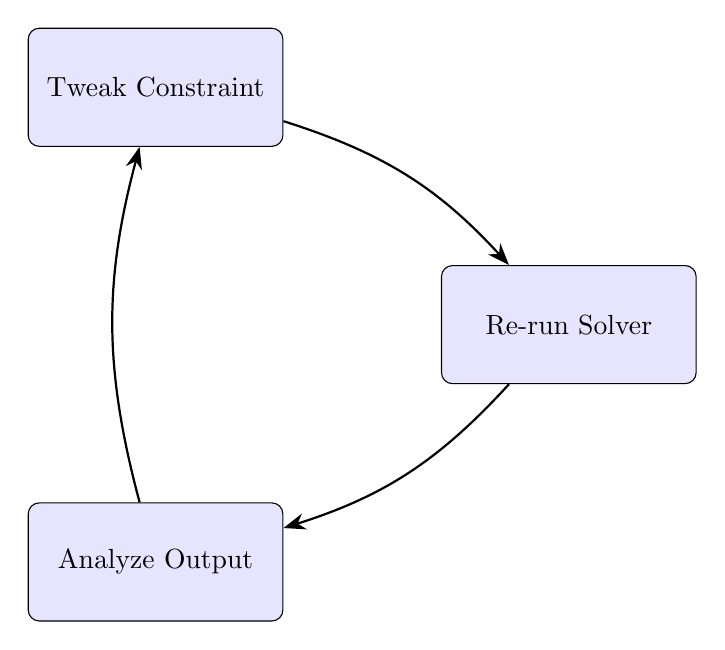
\begin{tikzpicture}[
      node distance=1.5cm and 2cm,
      box/.style={rectangle, draw, fill=blue!10, text width=3cm, text centered, rounded corners, minimum height=1.5cm},
      arrow/.style={-{Stealth[scale=1.2]}, thick}
    ]
      \node[box] (tweak) {Tweak Constraint};
      \node[box, below right=of tweak] (rerun) {Re-run Solver};
      \node[box, below left=of rerun] (analyze) {Analyze Output};
      
      \draw[arrow] (tweak) to[bend left=15] (rerun);
      \draw[arrow] (rerun) to[bend left=15] (analyze);
      \draw[arrow] (analyze) to[bend left=15] (tweak);
    \end{tikzpicture}
  \end{center}
\end{frame}

\begin{frame}{Scenario 1 - The Protein Bulking Phase}
  \begin{center}
    \Large
    Protein Constraint:
    
    \vspace{0.5cm}
    50g \hspace{1cm} $\longrightarrow$ \hspace{1cm} \textbf{150g}
    \vspace{1cm}
    
    \normalsize
    \begin{columns}
      \column{0.5\textwidth}
      \centering
      Total Daily Cost?
      
      (Up, Down, Same)
      
      \column{0.5\textwidth}
      \centering
      Aggressive Additions?
      
      (Which menu items)
    \end{columns}
  \end{center}
\end{frame}

\begin{frame}{Solving Scenario 1 - The Results}
  \begin{columns}
    \column{0.5\textwidth}
    \begin{block}{Before (50g Protein)}
      \begin{itemize}
        \item High carbs
        \item Lower total cost
        \item Cheap fillers
      \end{itemize}
    \end{block}
    
    \column{0.5\textwidth}
    \begin{block}{After (150g Protein)}
      \begin{itemize}
        \item High protein
        \item Higher total cost
        \item McDoubles added
      \end{itemize}
    \end{block}
  \end{columns}
  
  \vspace{1cm}
  \centering
  \textbf{Takeaways:}
  
  Tighter constraints = Higher costs
  
  Cheap fillers $\rightarrow$ Cost-effective protein
\end{frame}

\begin{frame}{Scenario 2 - The Calorie Deficit}
  \begin{center}
    \Large
    New Constraint:
    
    \vspace{0.5cm}
    Max Calories $\le$ \textbf{1,500 kcal}
    \vspace{1cm}
    
    \normalsize
    \begin{columns}
      \column{0.5\textwidth}
      \centering
      Mathematically possible?
      
      \column{0.5\textwidth}
      \centering
      Shift to nutrient-dense?
    \end{columns}
  \end{center}
\end{frame}

\begin{frame}{Solving Scenario 2 - Feasibility Reality Check}
  \begin{center}
    \textbf{\Large INFEASIBLE}
    
    \vspace{0.5cm}
    \textit{No mathematical combination satisfies all rules.}
    
    \vspace{1cm}
    \begin{columns}
      \column{0.5\textwidth}
      \begin{block}{The Reality}
        You can't have it all.
      \end{block}
      
      \column{0.5\textwidth}
      \begin{block}{The Solution}
        Relax constraints (spend more, fewer vitamins).
      \end{block}
    \end{columns}
  \end{center}
\end{frame}

\section{Part 2: The 0-1 Knapsack Problem (Integer Linear Programming)}

\begin{frame}{A New Challenge - Integer Linear Programming (ILP)}
  \begin{columns}
    \column{0.5\textwidth}
    \centering
    \textbf{Continuous Variables}
    
    \vspace{0.5cm}
    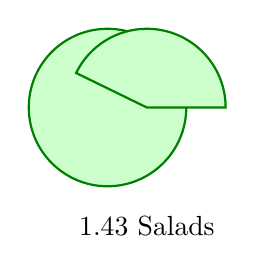
\begin{tikzpicture}
      \draw[fill=green!20, draw=green!50!black, thick] (0,0) circle (1cm);
      \draw[fill=green!20, draw=green!50!black, thick] (1.5,0) arc(0:154:1cm) -- (0.5,0) -- cycle;
      \node at (0.5, -1.5) {1.43 Salads};
    \end{tikzpicture}
    
    \column{0.5\textwidth}
    \centering
    \textbf{Binary (0/1) Variables}
    
    \vspace{0.5cm}
    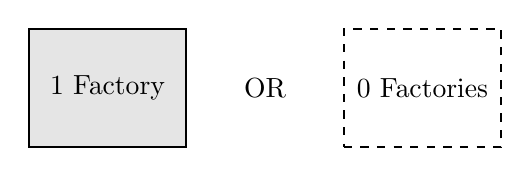
\begin{tikzpicture}
      \node[draw=black, thick, fill=gray!20, minimum width=2cm, minimum height=1.5cm] at (0,0) {1 Factory};
      \node at (2,0) {OR};
      \node[draw=black, thick, dashed, minimum width=2cm, minimum height=1.5cm] at (4,0) {0 Factories};
    \end{tikzpicture}
  \end{columns}
\end{frame}

\begin{frame}{The Hiking Dilemma}
  \begin{center}
    \Huge \textbf{0-1 Knapsack Problem}
    
    \vspace{1cm}
    \Large
    \textbf{Goal:} Maximize Survival Value
    
    \vspace{0.5cm}
    \textbf{Limit:} 10 lbs Maximum
  \end{center}
\end{frame}

\begin{frame}{Meet Your Gear (The Data)}
  \begin{center}
    \Large
    \renewcommand{\arraystretch}{1.5}
    \begin{tabular}{|l|c|c|}
      \hline
      \textbf{Item} & \textbf{Value} & \textbf{Weight (lbs)} \\
      \hline
      Tent & 10 & 5 \\
      \hline
      Stove & 40 & 4 \\
      \hline
      Water Filter & 30 & 6 \\
      \hline
      Sleeping Bag & 50 & 7 \\
      \hline
    \end{tabular}
  \end{center}
\end{frame}

\begin{frame}{Translating the Backpack into Google Sheets}
  \begin{center}
    \renewcommand{\arraystretch}{1.2}
    \resizebox{\linewidth}{!}{%
    \begin{tabular}{|c|l|c|c|c|}
      \hline
      & \textbf{A} & \textbf{B} & \textbf{C} & \textbf{D} \\
      \hline
      \textbf{1} & \textbf{Item} & \textbf{Value} & \textbf{Weight} & \textbf{Pack It?} \\
      \hline
      \textbf{2} & Tent & 10 & 5 & 0 \\
      \hline
      \textbf{3} & Stove & 40 & 4 & 0 \\
      \hline
      \textbf{4} & Water Filter & 30 & 6 & 0 \\
      \hline
      \textbf{5} & Sleeping Bag & 50 & 7 & 0 \\
      \hline
      \multicolumn{5}{c}{} \\
      \hline
      \textbf{7} & \textbf{Totals} & \textbf{=SUMPRODUCT(B2:B5, D2:D5)} & \textbf{=SUMPRODUCT(C2:C5, D2:D5)} & \\
      \hline
    \end{tabular}%
    }
  \end{center}
\end{frame}

\begin{frame}{Solving with OpenSolver (The Magic of \texttt{bin})}
  \Large
  \begin{enumerate}
    \item \textbf{Objective:} Maximize Total Value
    \vspace{0.5cm}
    \item \textbf{Constraint:} Total Weight $\le$ 10
    \vspace{0.5cm}
    \item \textbf{Variables:} \texttt{bin} (Binary 0 or 1)
  \end{enumerate}
  
  \vspace{1cm}
  \normalsize
  \centering
  \textbf{Optimal Solution:}
  
  Stove (4 lbs) + Water Filter (6 lbs) = 10 lbs (Value: 70)
\end{frame}


\begin{frame}{Next Class Preview}
\frametitle{Next Class Preview}
\begin{itemize}
  \item Python optimization next week!
  \item Bring your curiosity.
  \item Homework due: Practice this problem.
  \item Engage: Prep a question for next time!
\end{itemize}
\end{frame}



\end{document}